
% v2-acmsmall-sample.tex, dated March 6 2012
% This is a sample file for ACM small trim journals
%
% Compilation using 'acmsmall.cls' - version 1.3 (March 2012), Aptara Inc.
% (c) 2010 Association for Computing Machinery (ACM)
%
% Questions/Suggestions/Feedback should be addressed to => "acmtexsupport@aptaracorp.com".
% Users can also go through the FAQs available on the journal's submission webpage.
%
% Steps to compile: latex, bibtex, latex latex
%
% For tracking purposes => this is v1.3 - March 2012
\documentclass[prodmode,acmtecs]{acmsmall} % Aptara syntax
\usepackage[spanish,polish]{babel}
\usepackage[T1]{fontenc}
\usepackage{fancyvrb}
\usepackage{graphicx,hyperref}
\newcommand\cutout[1]{}


\usepackage[table]{xcolor}
\usepackage[utf8]{inputenc}
\usepackage[parfill]{parskip}
\usepackage{tabulary}
\PassOptionsToPackage{hyphens}{url}
\usepackage{hyperref}    
\usepackage[capitalize]{cleveref}


% Metadata Information
% !!! TODO: SET THESE VALUES !!!
\acmVolume{0}
\acmNumber{0}
\acmArticle{CFP}
\acmYear{0}
\acmMonth{0}

\newcounter{colstart}
\setcounter{page}{4}

\RecustomVerbatimCommand{\VerbatimInput}{VerbatimInput}%
{
%fontsize=\footnotesize,
fontfamily=\rmdefault
}


\newcommand{\UnderscoreCommands}{%\do\verbatiminput%
\do\citeNP \do\citeA \do\citeANP \do\citeN \do\shortcite%
\do\shortciteNP \do\shortciteA \do\shortciteANP \do\shortciteN%
\do\citeyear \do\citeyearNP%
}

\usepackage[strings]{underscore}



% Document starts
\begin{document}


\setcounter{colstart}{\thepage}

\acmArticle{CFP}
\title{\huge\sc SIGLOG Monthly 215}
\author{DAVID PURSER\affil{Max Planck Institute for Software Systems, Saarbr\"ucken}
\vspace*{-2.6cm}\begin{flushright}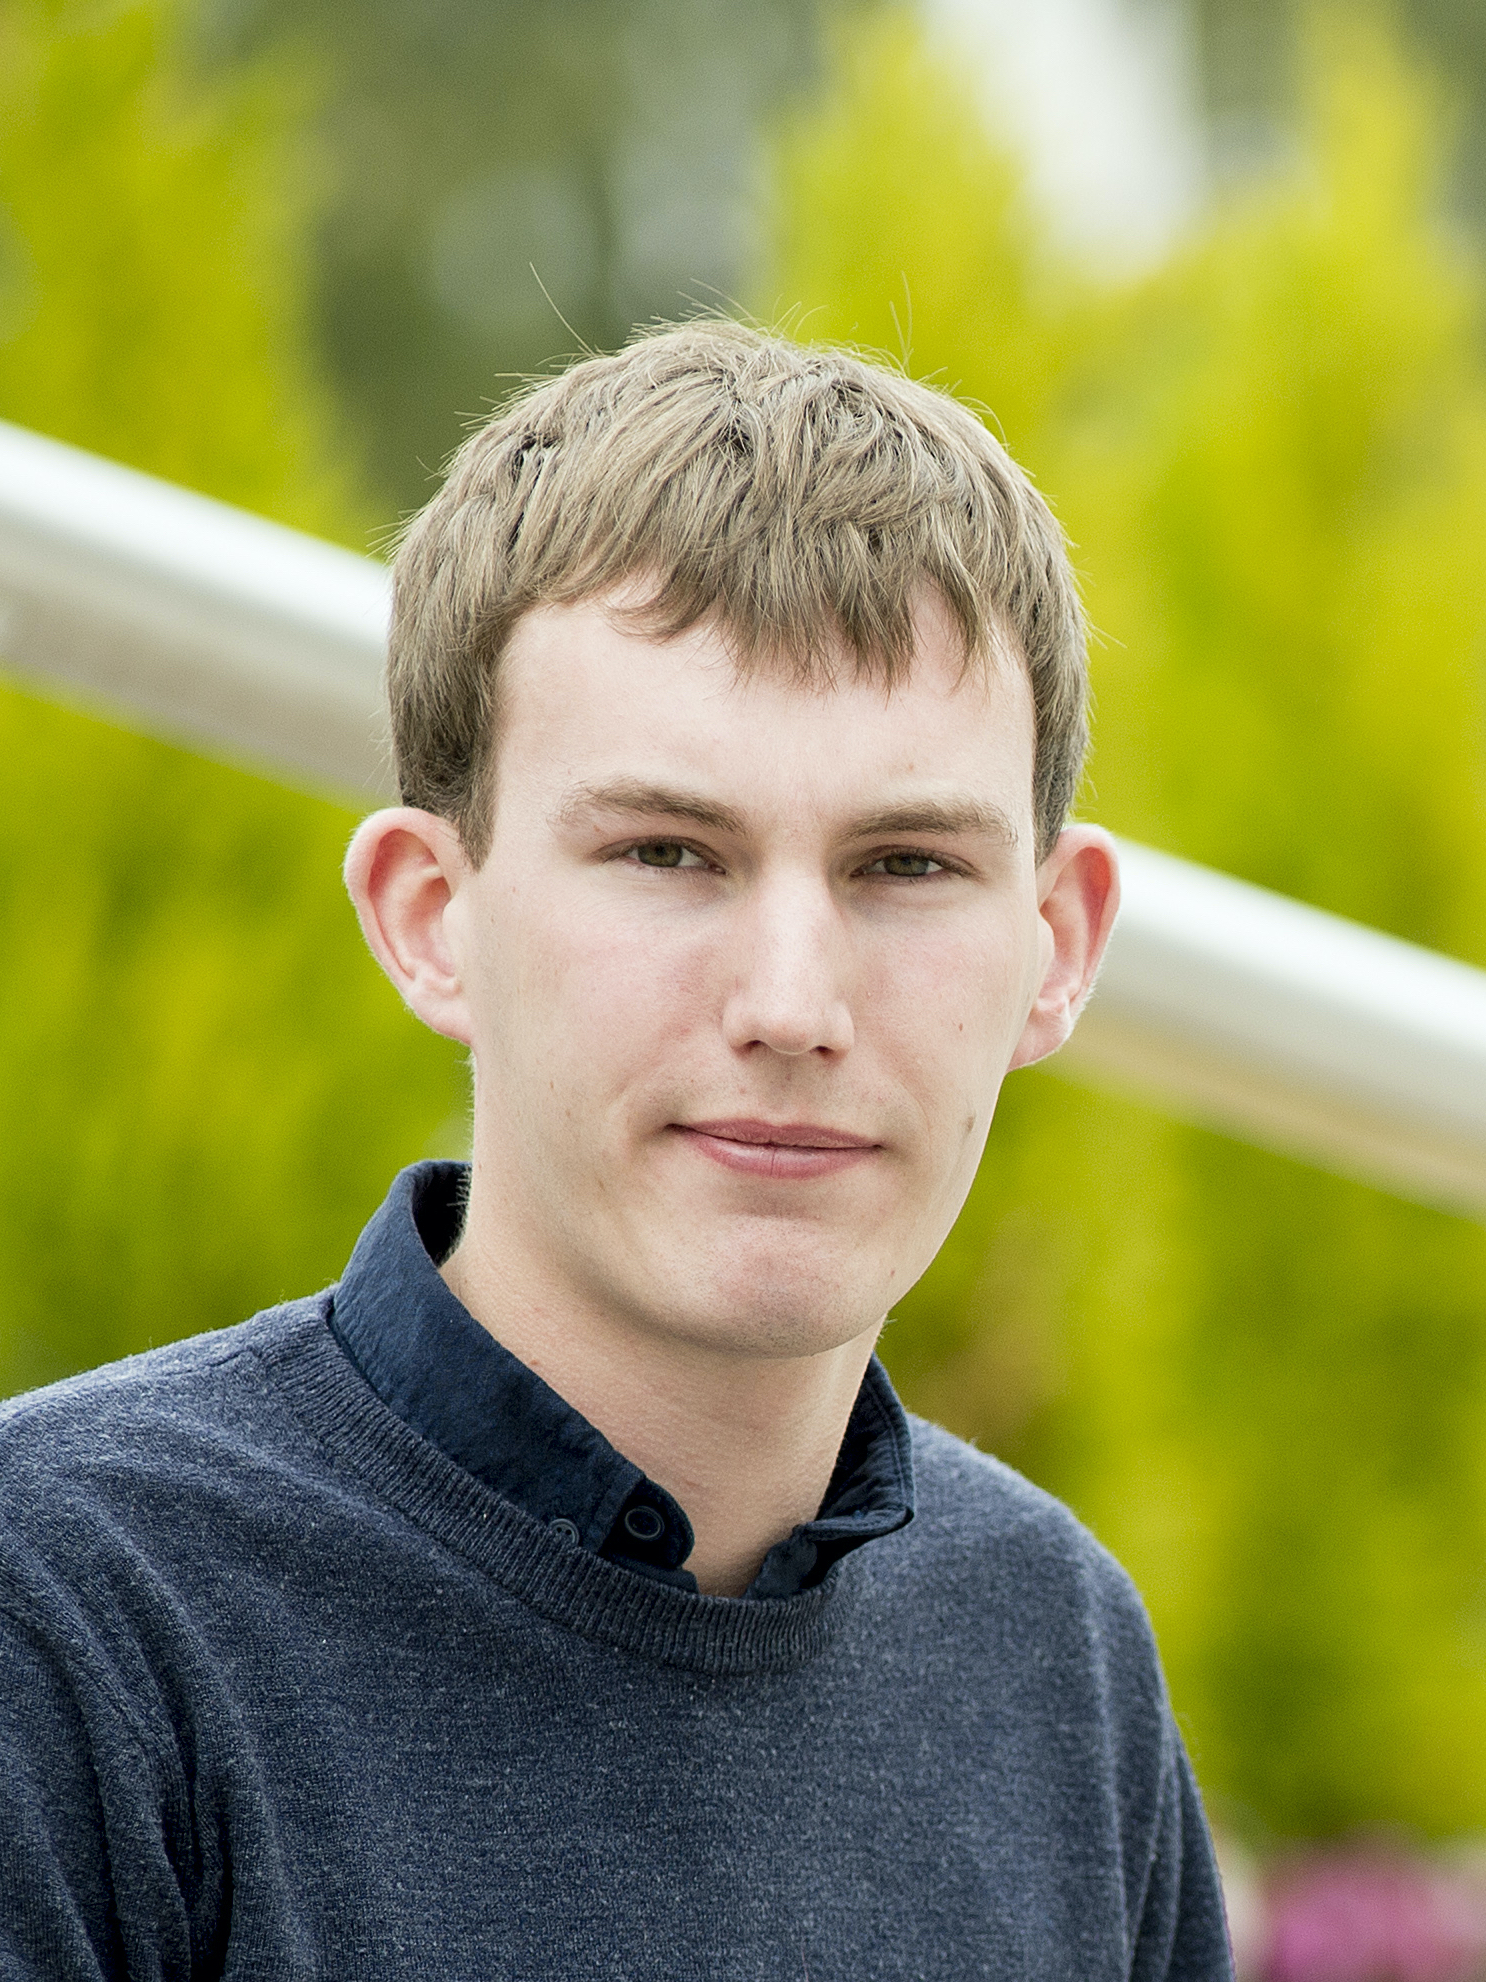
\includegraphics[width=30mm]{dp}\end{flushright}
}

\maketitlee

\href{https://lics.siglog.org/newsletters/}{Past Issues}
 - 
\href{https://lics.siglog.org/newsletters/inst.html}{How to submit an announcement}
\section{Table of Content}\begin{itemize}\item DEADLINES (\cref{deadlines}) 
 
\item CALLS 
 
\begin{itemize}\item XLoKR 2021 (CALL FOR PAPERS) (\cref{XLoKR2021})
\item FSCD 2021 (CALL FOR PARTICIPATION) (\cref{FSCD2021})
\item SPIN 2021 (CALL FOR PARTICIPATION) (\cref{SPIN2021})
\item FMM 2021 (CALL FOR PAPERS) (\cref{FMM2021})
\item FSTTCS 2021 (CALL FOR PAPERS) (\cref{FSTTCS2021})
\item CPP 2022 (CALL FOR PAPERS) (\cref{CPP2022})
\item FLoC 2022 (CALL FOR WORKSHOPS) (\cref{FLoC2022})
\end{itemize} 
\end{itemize}\section{Deadlines}\label{deadlines}\rowcolors{1}{white}{gray!25}\begin{tabulary}{\linewidth}{LL}ACKERMANN AWARD 2021:  & Jul 01, 2021 (Deadline for nomination) \\
NMR-2021:  & Jul 2, 2021 (Paper registration, Extended), Jul 7, 2021 (Paper, Extended) \\
XLoKR 2021:  & Jul 02, 2021 (Paper) \\
CSL 2022:  & Jul 05, 2021 (Abstract), Jul 12, 2021 (Paper) \\
OVERLAY 2021:  & Jul 11, 2021 (Paper) \\
FSCD 2021:  & Jul 11, 2021 (Registration deadline) \\
CPSIoTSec 2021:  & Jul 13, 2021 (Submission deadline, Extended), Jul 30, 2021 (Submission deadline only for papers rejected from ACM CCS 2021) \\
FMM 2021:  & Jul 14, 2021 (Paper) \\
FSTTCS 2021:  & Jul 19, 2021 (Submission deadline (firm)) \\
RW 2021:  & Aug 25, 2021 (Registration closes) \\
CCC 2021:  & Aug 30, 2021 (Deadline) \\
CPP 2022:  & Sep 16, 2021 (Abstract Submission Deadline) \\
FLoC 2022:  & Sep 27, 2021 (Submission of workshop proposals deadline) \\
\end{tabulary}
\section{XLoKR 2021: 2nd Workshop on Explainable Logic-Based Knowledge Representation (XLoKR 2021) }\label{XLoKR2021}  co-located with KR 2021 \href{https://kr2021.kbsg.rwth-aachen.de}{https://kr2021.kbsg.rwth-aachen.de}\\ 
  6-8 November 2021 (exact date(s) TBD), Hanoi, Vietnam (virtually) \\ 
  \href{https://xlokr21.ai.vub.ac.be/}{https://xlokr21.ai.vub.ac.be/} \\ 
CALL FOR PAPERS 

\begin{itemize}\item   Embedded or cyber-physical systems that interact autonomously with the real world, or with users they are supposed to support, must continuously make decisions based on sensor data, user input, knowledge they have acquired during runtime as well as knowledge provided during design-time. To make the behavior of such systems comprehensible, they need to be able to explain their decisions to the user or, after something has gone wrong, to an accident investigator. 
 
  While systems that use Machine Learning (ML) to interpret sensor data are very fast and usually quite accurate, their decisions are notoriously hard to explain, though huge efforts are currently being made to overcome this problem. In contrast, decisions made by reasoning about symbolically represented knowledge are in principle easy to explain. For example, if the knowledge is represented in (some fragment of) first-order logic, and a decision is made based on the result of a first-order reasoning process, then one can in principle use a formal proof in an appropriate calculus to explain a positive reasoning result, and a counter-model to explain a negative one. In practice, however, things are not so easy also in the symbolic KR setting. For example, proofs and counter-models may be very large, and thus it may be hard to comprehend why they demonstrate a positive or negative reasoning result, in particular for users that are not experts in logic. Thus, to leverage explainability as an advantage of symbolic KR over ML-based approaches, one needs to ensure that explanations can really be given in a way that is comprehensible to different classes of users (from knowledge engineers to laypersons).  
 
  The problem of explaining why a consequence does or does not follow from a given set of axioms has been considered for full first-order theorem proving since at least 40 years, but there usually with mathematicians as users in mind. In knowledge representation and reasoning, efforts in this direction are more recent, and were usually restricted to sub-areas of KR such as AI planning and description logics. The purpose of this workshop is to bring together researchers from different sub-areas of KR and automated deduction that are working on explainability in their respective fields, with the goal of exchanging experiences and approaches. A non-exhaustive list of areas to be covered by the workshop are the following: AI planning Answer set programming Argumentation frameworks Automated reasoning Causal reasoning Constraint programming Description logics Non-monotonic reasoning Probabilistic representation and reasoning  
 
\item  INVITED SPEAKERS 
 
  Sheila McIlraith and Joe Halpern will deliver the keynotes at the workshop.  
 
\item  IMPORTANT DATES   
 
\rowcolors{1}{white}{gray!25}\begin{tabulary}{\linewidth}{LL}Paper submission:  & Jul 02, 2021 \\
Notification:  & Aug 06, 2021 \\
Workshop dates (exact date TBD):  & Nov 6-8, 2021 \\
\end{tabulary}
 
\item   SUBMISSION INFORMATION 
 
  Researchers interested in participating in the workshop should submit extended abstracts of 2-5 pages in Springer LNCS Style on topics related to explanation in logic-based KR: \href{https://easychair.org/conferences/?conf=xlokr21}{https://easychair.org/conferences/?conf=xlokr21}.  
 
  The workshop will have informal proceedings, and thus, in addition to new work, also papers covering results that have recently been published or will be published at other venues are welcome.  
 
\end{itemize}\section{FSCD 2021: Sixth International Conference on Formal Structures for Computation and Deduction}\label{FSCD2021}  July 17 – July 24, 2021, Buenos Aires, Argentina\\ 
  \href{https://fscd2021.github.io/}{https://fscd2021.github.io/}\\ 
  In-cooperation with ACM SIGLOG and SIGPLAN\\ 
CALL FOR PARTICIPATION 

\begin{itemize}\item  The 2021 edition of FSCD and of its satellite workshops will be held online. Participation will, a priori, be free of charge, unless we receive way too many requests, in which case we will invite those who can to pay the modest amount of 7 USD. 
 
  FSCD covers all aspects of formal structures for computation and deduction from theoretical foundations to applications. Building on two communities, RTA (Rewriting Techniques and Applications) and TLCA (Typed Lambda Calculi and Applications), FSCD embraces their core topics and broadens their scope to closely related areas in logics, models of computation (e.g., quantum computing, probabilistic computing, homotopy type theory), semantics and verification in new challenging areas (e.g., blockchain protocols or deep learning algorithms). 
 
\item  REGISTRATION  
 
  Open at: \href{https://fscd2021.dc.uba.ar/registration.html}{https://fscd2021.dc.uba.ar/registration.html} 
 
  This link should be used also to register for affiliated workshops. 
 
Registration deadline: Jul 11, 2021 
 
  FSCD 2021 will run over the Clowdr platform. After the registration is closed, you will receive an invitation link and instructions on how to participate. 
 
\item  INVITED SPEAKERS   
 
\begin{itemize}\item  Zena M. Ariola \href{https://ix.cs.uoregon.edu/}{https://ix.cs.uoregon.edu/}~ariola/ 
\item  Nao Hirokawa \href{https://www.jaist.ac.jp/}{https://www.jaist.ac.jp/}~hirokawa/ 
\item  Elaine Pimentel \href{https://sites.google.com/site/elainepimentel/}{https://sites.google.com/site/elainepimentel/} 
\item  Sam Staton \href{https://www.cs.ox.ac.uk/people/samuel.staton/main.html}{https://www.cs.ox.ac.uk/people/samuel.staton/main.html}
\end{itemize} 
\item  FSCD AFFILIATED WORKSHOPS:   
 
\begin{itemize}\item  HoTT/UF (6th Workshop on Homotopy Type Theory/Univalent Foundations, July 17-18) 
\item  ITRS (10th Workshop on Intersection Types and Related Systems, July 17) 
\item  WPTE (7th International Workshop on Rewriting Techniques for Program Transformations and Evaluation, July 18) 
\item  UNIF (35th International Workshop on Unification, July 18) 
\item  LSFA (16th Logical and Semantics Frameworks with Applications, July 23-24) 
\item  IWC (10th International Workshop on Confluence, July 23) 
\item  IFIP WG 1.6 (24th meeting of the IFIP Working Group 1.6: Rewriting, July 24)
\end{itemize} 
\end{itemize}\section{SPIN 2021: International Symposium on Model Checking of Software}\label{SPIN2021}  July 12, 2021, 9:50 to 18:15 CEST\\ 
  ONLINE EVENT\\ 
  \href{https://conf.researchr.org/home/spin-2021}{https://conf.researchr.org/home/spin-2021}\\ 
CALL FOR PARTICIPATION 

\begin{itemize}\item  ABOUT SPIN 
 
  The 27th edition of the SPIN symposium aims at bringing together researchers and practitioners interested in automated tool-based techniques for the analysis of software as well as models of software, for the purpose of verification and validation. The symposium specifically focuses on concurrent software but does not exclude the analysis of sequential software. Submissions are solicited on theoretical results, novel algorithms (classical and quantum), tool development, including for modern hardware (parallel and distributed), and empirical evaluation. 
 
\item  REGISTRATION 
 
  Registration is free. In order to receive the event links, sign up here: \href{https://conf.researchr.org/home/spin-2021#Registration}{https://conf.researchr.org/home/spin-2021\#Registration} 
 
\item  INVITED SPEAKERS  
 
\begin{itemize}\item  Vincenzo Ciancia, ISTI-CNR 
\item  Mariëlle Stoelinga, Twente / Radboud University 
\item  Moshe Vardi, Rice University
\end{itemize} 
\end{itemize}\section{FMM 2021: Fifth Workshop on Formal Mathematics for Mathematicians}\label{FMM2021}  26-31 July 2021 (exact date TBA) Timisoara, Romania (hybrid or fully virtual) \href{https://cicm-conference.org/2021/cicm.php?event=fmm}{https://cicm-conference.org/2021/cicm.php?event=fmm}  \\ 
  Co-located with 14th Conference on Intelligent Computer Mathematics (CICM 2021) \href{https://cicm-conference.org/2021/cicm.php}{https://cicm-conference.org/2021/cicm.php}\\ 
CALL FOR PAPERS 

\begin{itemize}\item  DATES 
 
\rowcolors{1}{white}{gray!25}\begin{tabulary}{\linewidth}{LL}Paper submission:  & Jul 14, 2021 \\
Author notification:  & Jul 21, 2021 \\
Final version due:  & Jul 25, 2021 \\
\end{tabulary}
 
\item  SCOPE 
 
  The FMM workshop series enables mathematicians interested in computer assistance and researchers in formal and computer-understandable mathematics to meet and exchange ideas. The meeting provides a platform for discussion of suitable forms of computer assistance between the formal community and interested mathematicians and other researchers. 
 
  The main points of interest include:  
 
\begin{itemize}\item  formalization of challenging mathematical problems   
\item  design of proof languages and techniques   
\item  repositories of formalized mathematics   
\item  interactive and automated theorem proving   
\item  development of proof assistants   
\item  semantic representation of mathematical knowledge   
\item  formal tools in program verification   
\item  foundations and philosophy of mathematics   
\item  proof assistants in education 
\end{itemize} 
\item  INVITED SPEAKERS  
 
  Mario Carneiro (Carnegie Mellon University, USA) Manuel Eberl (Technical University of Munich, Germany)  
 
\item  SUBMISSION GUIDELINES 
 
 \href{https://easychair.org/conferences/?conf=cicm2021}{https://easychair.org/conferences/?conf=cicm2021} and choose FMM.  
 
 We welcome submission of short papers presenting research related to the workshop's points of interest. Submitted papers should be 4-6 pages long and formatted in LaTeX using the style ``onecolceurws'' (see \href{http://ceur-ws.org/Vol-XXX/samplestyles/}{http://ceur-ws.org/Vol-XXX/samplestyles/}). 
 
 Submission is continuous until 14 July 2021 AoE. At least one author of each accepted paper is expected to attend FMM and present the work (online or in person). We plan to publish electronic proceedings in the CEUR Workshop Proceedings series.  
 
\end{itemize}\section{FSTTCS 2021: Foundations of Software Technology and Theoretical Computer Science}\label{FSTTCS2021}  December 15 - 18, 2021\\ 
  Virtual Conference\\ 
  \href{https://www.fsttcs.org.in/2021/}{https://www.fsttcs.org.in/2021/}\\ 
CALL FOR PAPERS 

\begin{itemize}\item  FSTTCS 2021 is the 41’st conference on Foundations of Software Technology and Theoretical Computer Science. It is organised by IARCS, the Indian Association for Research in Computing Science. It is a forum for presenting original results in foundational aspects of Computer Science and Software Technology. 
 
\item  LIST OF TOPICS 
 
  Track A 
 
\begin{itemize}\item  Algebraic Complexity
\item  Algorithms and Data Structures
\item  Algorithmic Graph Theory and Combinatorics
\item  Approximation Algorithms
\item  Combinatorial Optimization
\item  Communication Complexity
\item  Computational Biology
\item  Computational Complexity
\item  Computational Geometry
\item  Computational Learning Theory
\item  Cryptography and Security
\item  Data Streaming and Sublinear algorithms
\item  Economics and Computation
\item  Parallel, Distributed and Online Algorithms
\item  Parameterized Complexity
\item  Proof Complexity
\item  Quantum Computing
\item  Randomness in Computing
\item  Theoretical Aspects of Mobile and High-Performance Computing
\end{itemize} 
  Track B 
 
\begin{itemize}\item  Automata, Games and Formal Languages
\item  Logic in Computer Science
\item  Modal and Temporal Logics
\item  Models of Concurrent, Distributed and Mobile Systems
\item  Models of Timed, Reactive, Hybrid and Stochastic Systems
\item  Model Theory
\item  Principles and Semantics of Programming Languages
\item  Program Analysis and Transformation
\item  Security Protocols
\item  Specification, Verification and Synthesis
\item  Theorem Proving and Decision Procedures
\end{itemize} 
\item  INVITED SPEAKERS 
 
\begin{itemize}\item  Scott Aaronson (University of Texas, Austin)
\item  Javier Esparza (TU Munich)
\item  Leslie Ann Goldberg (University of Oxford)
\item  Huijia (Rachel) Lin (University of Washington)
\item  Rahul Savani (University of Liverpool)
\end{itemize} 
\item  WORKSHOPS AND CO-LOCATED EVENTS 
 
  See conference website for the most recent information. We invite researchers interested in holding a workshop or co-located event to contact the PC Chairs. 
 
\item  SUBMISSION GUIDELINES 
 
  \href{https://easychair.org/conferences/?conf=fsttcs2021}{https://easychair.org/conferences/?conf=fsttcs2021} 
 
  LIPIcs LaTeX style, 12 pages excluding bibliography but may include a clearly marked appendix containing technical details. The appendix will be read only at the discretion of the program committee. Simultaneous submissions to journals or other conferences with published proceedings are disallowed. Accepted papers published in LIPIcs (open access CC-BY) subject to one author presenting the paper at the conference. 
 
\item  IMPORTANT DATES (AoE) 
 
\rowcolors{1}{white}{gray!25}\begin{tabulary}{\linewidth}{LL}Submission deadline (firm):  & Jul 19, 2021 \\
Rebuttal phase:  & Aug 30 - Sept 1, 2021 \\
Notification to authors:  & Sep 20, 2021 \\
Deadline for camera-ready papers:  & Oct 04, 2021 \\
Pre-conference workshops:  & Dec 14, 2021 \\
FSTTCS 2021:  & December 15–17, 2021 \\
Post-conference workshops:  & Dec 18, 2021 \\
\end{tabulary}
 
\end{itemize}\section{CPP 2022: Certified Programs and Proofs}\label{CPP2022}  16-18 January 2022\\ 
  Co-located with POPL 2022 in Philadelphia, Pennsylvania, United States\\ 
  \href{https://popl22.sigplan.org/home/CPP-2022}{https://popl22.sigplan.org/home/CPP-2022}\\ 
CALL FOR PAPERS 

\begin{itemize}\item  Certified Programs and Proofs (CPP) is an international conference on practical and theoretical topics in all areas that consider formal verification and certification as an essential paradigm for their work. CPP spans areas of computer science, mathematics, logic, and education. 
 
  CPP 2022 is sponsored by ACM SIGPLAN, in cooperation with ACM SIGLOG. 
 
  CPP 2022 will welcome contributions from all members of the community. The CPP 2022 organizers will strive to enable both in-person and remote participation, in cooperation with the POPL 2022 organizers.  
 
\item  IMPORTANT DATES (AoE, strict) 
 
\rowcolors{1}{white}{gray!25}\begin{tabulary}{\linewidth}{LL}Abstract Submission Deadline:  & Sep 16, 2021 \\
Paper Submission Deadline:  & Sep 22, 2021 \\
Notification (tentative):  & Nov 22, 2021 \\
Camera Ready Deadline (tentative):  & Dec 12, 2021 \\
Conference:  & Jan 16-18 2022 \\
\end{tabulary}
 
\item  DISTINGUISHED PAPER AWARDS 
 
  Around 10% of the accepted papers at CPP 2022 will be designated as Distinguished Papers. This award highlights papers that the CPP program committee thinks should be read by a broad audience due to their relevance, originality, significance and clarity. 
 
\item  TOPICS OF INTEREST 
 
  We welcome submissions in research areas related to formal certification of programs and proofs. The following is a non-exhaustive list of topics of interest to CPP:  
 
\begin{itemize}\item  certified or certifying programming, compilation, linking, OS kernels, runtime systems, security monitors, and hardware; 
\item  certified mathematical libraries and mathematical theorems; 
\item  proof assistants (e.g, ACL2, Agda, Coq, Dafny, F*, HOL4, HOL Light, Idris, Isabelle, Lean, Mizar, Nuprl, PVS, etc); 
\item  new languages and tools for certified programming; 
\item  program analysis, program verification, and program synthesis; 
\item  program logics, type systems, and semantics for certified code; 
\item  logics for certifying concurrent and distributed systems; 
\item  mechanized metatheory, formalized programming language semantics, and logical frameworks; 
\item  higher-order logics, dependent type theory, proof theory, logical systems, separation logics, and logics for security; 
\item  verification of correctness and security properties; 
\item  formally verified blockchains and smart contracts; 
\item  certificates for decision procedures, including linear algebra, polynomial systems, SAT, SMT, and unification in algebras of interest; 
\item  certificates for semi-decision procedures, including equality, first-order logic, and higher-order unification; 
\item  certificates for program termination; 
\item  formal models of computation; 
\item  mechanized (un)decidability and computational complexity proofs; 
\item  formally certified methods for induction and coinduction; 
\item  integration of interactive and automated provers; 
\item  logical foundations of proof assistants; 
\item  applications of AI and machine learning to formal certification; 
\item  user interfaces for proof assistants and theorem provers; 
\item  teaching mathematics and computer science with proof assistants.
\end{itemize} 
\item  SUBMISSION GUIDELINES 
 
   Anonymized, English, ACM SIGPLAN (acmart sigplan option), PDF:  \href{https://cpp2022.hotcrp.com}{https://cpp2022.hotcrp.com} 
 
   Must provide sufficient detail to allow the program committee to assess the merits of the contribution.  
 
   Max 12 pages (excluding bibliography and appendices). The papers should be self-contained without the appendices. Shorter papers are welcome and will be given equal consideration. 
 
   Please see full CFP for full double-blind reviewing process, concurrent submissions, plagiarism, publications, copyright and open access. 
 
\end{itemize}\section{FLoC 2022: The 2022 Federated Logic Conference}\label{FLoC2022}  July 31 - August 12, 2022\\ 
  Haifa, Israel\\ 
  \href{http://www.floc2022.org/}{http://www.floc2022.org/}\\ 
CALL FOR WORKSHOPS 

\begin{itemize}\item  The Eighth Federated Logic Conference (FLoC 2022) will host the following ten conferences and affiliated workshops. 
 
\begin{itemize}\item  LICS (37th Annual ACM/IEEE Symposium on Logic in Computer Science)  \href{http://lics.rwth-aachen.de/}{http://lics.rwth-aachen.de/} Workshop chair: Frederic Blanqui Frederic.Blanqui@inria.fr
\item  FSCD (7th International Conference on Formal Structures for Computation and Deduction)  \href{http://fscd-conference.org/}{http://fscd-conference.org/} Workshop chair: Nachum Dershowitz nachumd@tau.ac.il
\item  ITP (13th International Conference on Interactive Theorem Proving)  \href{https://itp-conference.github.io/}{https://itp-conference.github.io/} Workshop chair: Cyril Cohen cyril.cohen@inria.fr
\item  IJCAR (International Joint Conference on Automated Reasoning) \href{http://www.ijcar.org}{http://www.ijcar.org} Workshop chair: Simon Robillard simon.robillard@imt-atlantique.fr
\item  CSF (35th IEEE Computer Security Foundations Symposium)  \href{http://www.ieee-security.org/CSFWweb/}{http://www.ieee-security.org/CSFWweb/} Workshop chair: Musard Balliu musard@kth.se
\item  CAV (34th International Conference on Computer Aided Verification) \href{http://i-cav.org/}{http://i-cav.org/} Workshop chair: TBD
\item  KR (19th International Conference on Principles of Knowledge Representation and Reasoning) \href{http://www.kr.org/}{http://www.kr.org/} Workshop chair: Stefan Borgwardt stefan.borgwardt@tu-dresden.de
\item  ICLP (38th International Conference on Logic Programming)  \href{https://www.cs.nmsu.edu/ALP/conferences/}{https://www.cs.nmsu.edu/ALP/conferences/} Workshop chair: Daniela Inclezan inclezd@miamioh.edu
\item  SAT (25th International Conference on Theory and Applications of Satisfiability Testing)  \href{http://www.satisfiability.org}{http://www.satisfiability.org} Workshop chair: TBD
\item  CP (25th International Conference on Principles and Practice of Constraint Programming)  \href{http://a4cp.org/events/cp-conference-series}{http://a4cp.org/events/cp-conference-series} Workshop chair: TBD
\end{itemize} 
\item  SUBMISSION OF WORKSHOP PROPOSALS 
 
  Researchers and practitioners are invited to submit proposals for workshops on topics in the field of computer science, related to logic in the broad sense. Each workshop proposal must indicate one affiliated conference of FLoC 2022. 
 
  It is strongly suggested that prospective workshop organizers contact the relevant conference workshop chair before submitting a proposal. 
 
  Each proposal should consist of the following two parts. 
 
  1) A short scientific justification of the proposed topic, its significance, and the particular benefits of the workshop to the community, as well as a list of previous or related workshops (if relevant).  
 
  2) An organisational part including: 
 
\begin{itemize}\item  contact information for the workshop organizers; 
\item  proposed affiliated conference; 
\item  estimate of the number of workshop participants (please note that small workshops, i.e., of less than ~13 participants, will likely be cancelled or merged); 
\item  proposed format and agenda (e.g. paper presentations, tutorials, demo sessions, etc.); 
\item  potential invited speakers; 
\item  procedures for selecting papers and participants; 
\item  plans for dissemination, if any (e.g. a journal special issue); 
\item  duration (which may vary from one day to two days); 
\item  preferred period (pre or post FLoC); 
\item  virtual/hybrid backup plans (including platform preference). 
\end{itemize} 
  The FLoC Organizing Committee will determine the final list of accepted workshops based on the recommendations from the Workshop Chairs of the hosting conferences and availability of space and facilities. 
 
  Proposals should be submitted through EasyChair: \href{https://easychair.org/conferences/?conf=floc2022workshops}{https://easychair.org/conferences/?conf=floc2022workshops} 
 
\item  IMPORTANT DATES 
 
\rowcolors{1}{white}{gray!25}\begin{tabulary}{\linewidth}{LL}Submission of workshop proposals deadline:  & Sep 27, 2021 \\
Notification:  & Nov 01, 2021 \\
Pre-FLoC workshops:  & Jul 31–Aug 1, 2022 \\
Post-FLoC workshops:  & Aug 11-12, 2022 \\
\end{tabulary}
 
\item  CONTACT INFORMATION 
 
  Questions regarding proposals should be sent to the workshop chairs of the proposed affiliated conference. General questions should be sent to: shaull@technion.ac.il GuillermoAlberto.Perez@uantwerpen.be 
 
\end{itemize}


To the \href{http://siglog.org/}{SIGLOG} or \href{https://lics.siglog.org}{LICS} website\end{document}